\documentclass[11pt]{scrartcl}

    \usepackage[ngerman]{babel}
    \usepackage{ucs}
    \usepackage[utf8x]{inputenc}
    \usepackage[T1]{fontenc}
    \usepackage{listings}
    \usepackage[usenames,dvipsnames]{xcolor}
    \usepackage{pict2e}
    \usepackage{graphicx}
    \usepackage[left=2.5cm,right=2.5cm,top=1.5cm,bottom=1cm,includeheadfoot]{geometry}
    \usepackage{amsmath}
    
    \input kvmacros

    % Define VHDL language for code snippets
    \lstdefinelanguage{VHDL}{
        morekeywords=[1]{
          library,use,all,entity,is,port,in,out,end,architecture,of,
          begin,and,or,Not,downto,ALL
        },
        morekeywords=[2]{
          STD_LOGIC_VECTOR,STD_LOGIC,IEEE,STD_LOGIC_1164,
          NUMERIC_STD,STD_LOGIC_ARITH,STD_LOGIC_UNSIGNED,std_logic_vector,
          std_logic
        },
        morecomment=[l]--
     }
     \colorlet{keyword}{blue}
     \colorlet{STD}{OrangeRed}
     \colorlet{comment}{OliveGreen}
     \lstdefinestyle{vhdl}{
        language     = VHDL,
        basicstyle   = \footnotesize \ttfamily,
        keywordstyle = [1]\color{keyword}\bfseries,
        keywordstyle = [2]\color{STD}\bfseries,
        commentstyle = \color{comment},
        breaklines   = true,
        tabsize      = 4,
        frame        = single
     }
     % End of VHDL definition

     % Define underline with color in formulas
    \newsavebox\MBox
    \newcommand\Cline[2][red]{{\sbox\MBox{$#2$}%
        \rlap{\usebox\MBox}\color{#1}\rule[-1.2\dp\MBox]{\wd\MBox}{0.5pt}}}

% -----------------------------------------------------------------------------------------
% Start document
\begin{document}
\title{Lösungen Aufgabensammlung K-1 bis K-10}
\author{Brice Dorsey Long Dje, Felix Jägers}
\maketitle

\section{Aufgabe K-1}

Gegebene Funktionstabelle f:

\begin{center}
\begin{tabular}{lr}
    \begin{tabular}[t]{r|cccc|c}
  ($i_{10}$)&$x$&$y$&$z$&$v$&$f$\\
  \hline
  0&0&0&0&0&0\\
  1&0&0&0&1&0\\
  2&0&0&1&0&1\\
  3&0&0&1&1&1\\
  4&0&1&0&0&1\\
  5&0&1&0&1&1\\
  6&0&1&1&0&0\\
  7&0&1&1&1&1\\
    \end{tabular}
  &
    \begin{tabular}[t]{r|cccc|c}
      ($i_{10}$)&$x$&$y$&$z$&$v$&$f$\\
  \hline
  8&1&0&0&0&0\\
  9&1&0&0&1&0\\
  10&1&0&1&0&1\\
  11&1&0&1&1&1\\
  12&1&1&0&0&1\\
  13&1&1&0&1&0\\
  14&1&1&1&0&0\\
  15&1&1&1&1&1\\
    \end{tabular}
\end{tabular}
\end{center}

Aus der Funktionstabelle erstelltes Karnaugh-Diagramme jeweils für DMF und KMF:

\begin{center}
\karnaughmap{4}{$f_{DMF}$:}{{$x$}{$y$}{$z$}{$v$}}
{0011110100111001}
{
    \put(1,2){\color{red}\circle{2}}
    \put(2,2){\color{green}\circle{2}}
    \put(3,3.5){\color{blue}\oval(1.9,1)[l]}
    \put(3,3.5){\color{blue}\oval(1.9,1)[r]}
    \put(3.5,0){\color{orange}\oval(1,1.9)[t]}
    \put(3.5,4){\color{orange}\oval(1,1.9)[b]}
}
\karnaughmap{4}{$f_{KMF}$:}{{$x$}{$y$}{$z$}{$v$}}
{0011110100111001}
{
    \put(1,4){\color{red}\oval(1.9,1.9)[b]}
    \put(1,0){\color{red}\oval(1.9,1.9)[t]}
    \put(3.5,2){\color{green}\oval(1,1.9)[b]}
    \put(3.5,2){\color{green}\oval(1,1.9)[t]}
    \put(2,0.5){\color{blue}\oval(1.9,1)[l]}
    \put(2,0.5){\color{blue}\oval(1.9,1)[r]}
}
\end{center}

\[f_{KMF} = (\overline{v} \lor z \lor \overline{x}) \land
 (z \lor y) \land (\overline{z} \lor \overline{y} \lor v) \]

\lstinputlisting[style=vhdl]{../Aufgabe_K-1/Labor1_1.vhd}

\newpage
\section{Aufgabe K-2}

Gegebene Funktionstabelle f aus dem Karnaugh-Diagramme abgelesen:\\

\begin{center}
\begin{tabular}{lr}
    \begin{tabular}[t]{r|cccc|c}
        ($i_{10}$)&$x$&$y$&$z$&$v$&$f$\\
        \hline
        0&0&0&0&0&0\\
        1&0&0&0&1&1\\
        2&0&0&1&0&1\\
        3&0&0&1&1&0\\
        4&0&1&0&0&1\\
        5&0&1&0&1&0\\
        6&0&1&1&0&0\\
        7&0&1&1&1&1\\
    \end{tabular}
  &
    \begin{tabular}[t]{r|cccc|c}
      ($i_{10}$)&$x$&$y$&$z$&$v$&$f$\\
        \hline
        8&1&0&0&0&1\\
        9&1&0&0&1&0\\
        10&1&0&1&0&0\\
        11&1&0&1&1&1\\
        12&1&1&0&0&0\\
        13&1&1&0&1&1\\
        14&1&1&1&0&1\\
        15&1&1&1&1&0\\
    \end{tabular}
\end{tabular}
\end{center}

% 1a) DNF erstellen ----------------------------
\subsection{a) DNF bestimmen}
\noindent Aus der Funktionstabelle die DNF erstellt:

\begin{align*}
    f_{DNF} =&
    \Cline[red]{(\overline{x} \land \overline{y} \land \overline{z} \land v)} \lor
    \Cline[red]{(\overline{x} \land \overline{y} \land z \land \overline{v})} \lor
    \Cline[green]{(x \land y \land z \land \overline{v})} \lor
    \Cline[green]{(x \land y \land \overline{z} \land v)} \lor\\
    &
    \Cline[blue]{(\overline{x} \land y \land z \land v)} \lor
    \Cline[blue]{(x \land \overline{y} \land z \land v)} \lor
    \Cline[orange]{(\overline{x} \land y \land \overline{z} \land \overline{v})} \lor
    \Cline[orange]{(x \land \overline{y} \land \overline{z} \land \overline{v})}\\
\end{align*}

% 1b) Beweis ----------------------------
\subsection{b) Beweis}
Ausklammern der gleichen Variablen innerhalb der jeweils gleich unterstrichenen Terme:

\begin{align*}
    f_{DNF} =&
    (\overline{x} \land \overline{y}) \lor
    \Cline[red]{((\overline{z} \land v) \lor (z \land \overline{v}))} \lor
    (x \land y) \lor
    \Cline[green]{((z \land \overline{v}) \lor (\overline{z} \land v))} \lor\\
    &
    (\overline{z} \land \overline{v}) \lor
    \Cline[blue]{((\overline{x} \land y) \lor (x \land \overline{y}))} \lor
    (z \land v) \lor
    \Cline[orange]{((x \land \overline{y}) \lor (\overline{x} \land y))}\\
\end{align*}

\noindent
Jeweils der unterstrichene Term ist ein XOR. Rot und Grün sind gleich und Blau und Orange.
Damit wird das auch direkt zusammen gefasst:

\begin{align*}
    f_{DNF} &=
    ((\overline{x} \land \overline{y}) \lor (x \land y)) \lor
    z \oplus v \lor
    ((\overline{z} \land \overline{v}) \lor (z \land v)) \lor
    x \oplus y\\
    &=
    (\overline{x \oplus y} \lor z \oplus v) \lor
    (x \oplus y \lor  \overline{z \oplus v})\\
    &=
    (x \oplus y \land  \overline{z \oplus v}) \lor
    (\overline{x \oplus y} \land z \oplus v)\\
    &=
    x \oplus y \oplus z \oplus v\\
\end{align*}

% 1c) Schaltung Minimalform ----------------------------
\subsection{c) Schaltung Minimalform}

Die Minimalform von einem XOR mit den zulässigen Gattern besteht aus einem NAND-, OR- und AND-Gatter.
Damit ist die Minimalform der gesamten Funktion drei von dieser XOR Realisierung verschaltet. Das sieht
dann folgendermaßen aus:
\begin{center}
    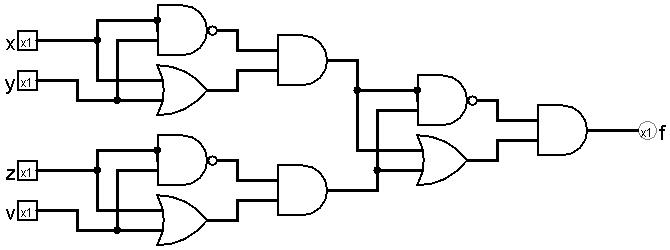
\includegraphics[width=0.7\textwidth]{../Aufgabe_K-2/Schaltung/Aufgabe_K-2.jpg}
\end{center}

\lstinputlisting[style=vhdl]{../Aufgabe_K-2/aufgabe_k2.vhd}

% Aufgabe K-4 -------------------------------------------------------------------
\newpage
\section{Aufgabe K-4}

Gegeben ist folgende Funktion:
\[f(x,y,z,v) = m_0 \lor m_2 \lor m_3 \lor m_4 \lor m_8 \lor m_{10} \lor m_{11} \lor m_{14} \lor m_{15}\]
Daraus werden die Tabelle und das Karnaugh- und das Veitch-Diagramm erstellt:

\begin{center}
\begin{tabular}{cc}
    \begin{tabular}[t]{r|cccc|c}
        ($i_{10}$)&$x$&$y$&$z$&$v$&$f$\\
        \hline
        0&0&0&0&0&1\\
        1&0&0&0&1&0\\
        2&0&0&1&0&1\\
        3&0&0&1&1&1\\
        4&0&1&0&0&1\\
        5&0&1&0&1&0\\
        6&0&1&1&0&0\\
        7&0&1&1&1&0\\
        8&1&0&0&0&1\\
        9&1&0&0&1&0\\
        10&1&0&1&0&1\\
        11&1&0&1&1&1\\
        12&1&1&0&0&0\\
        13&1&1&0&1&0\\
        14&1&1&1&0&1\\
        15&1&1&1&1&1\\
    \end{tabular}
    &
    \begin{tabular}[t]{c}
        Karnaugh-Diagramm für $f$:\\
        \karnaughmap{4}{$f_{K-DMF}$:}{{$x$}{$y$}{$z$}{$v$}}
        {1011100010110011}
        {
            \put(1,2){\color{red}\circle{2}}
            \put(1,1.5){\color{green}\oval(1.9,1)[l]}
            \put(1,2){\color{green}\line(1,0){2}}
            \put(1,1){\color{green}\line(1,0){2}}
            \put(3,1.5){\color{green}\oval(1.9,1)[r]}
            \put(0.5,3){\color{blue}\oval(1,1.9)[t]}
            \put(0,1){\color{blue}\line(0,1){2}}
            \put(1,1){\color{blue}\line(0,1){2}}
            \put(0.5,1){\color{blue}\oval(1,1.9)[b]}
            \put(4,3.5){\color{orange}\oval(1.9,1)[l]}
            \put(0,3.5){\color{orange}\oval(1.9,1)[r]}
        }\\
        Veitch-Diagramm für $f$:\\
        \veitchchart{4}{$f_{V-DMF}$:}{{$x$}{$y$}{$z$}{$v$}}
        {1011100010110011}
        {
            \put(1,2.5){\color{red}\oval(1.9,1)[l]}
            \put(1,2.5){\color{red}\oval(1.9,1)[r]}
            \put(1,0.5){\color{green}\oval(1.9,1)[l]}
            \put(1,1){\color{green}\line(1,0){2}}
            \put(1,0){\color{green}\line(1,0){2}}
            \put(3,0.5){\color{green}\oval(1.9,1)[r]}
            \put(0.5,3){\color{blue}\oval(1,1.9)[t]}
            \put(0,1){\color{blue}\line(0,1){2}}
            \put(1,1){\color{blue}\line(0,1){2}}
            \put(0.5,1){\color{blue}\oval(1,1.9)[b]}
            \put(2.5,0){\color{orange}\oval(1,1.9)[t]}
            \put(2.5,4){\color{orange}\oval(1,1.9)[b]}
        }
    \end{tabular}
\end{tabular}
\end{center}

\begin{align*}
    f_{K-DMF} &=
    (\overline{y} \land \overline{v}) \lor
    (\overline{y} \land z) \lor
    (x \land z) \lor
    (\overline{x} \land \overline{z} \land \overline{v})\\
    f_{V-DMF} &=
    (\overline{x} \land \overline{y} \land z) \lor
    (x \land z) \lor
    (\overline{y} \land \overline{v}) \lor
    (y \land \overline{v})\\
    &=
    (\overline{x} \land \overline{y} \land z) \lor
    (x \land z) \lor
    \overline{v}
\end{align*}

\end{document}